\documentclass[a4paper, 12pt]{article}

\usepackage{url}
\usepackage{graphicx}
\usepackage{caption}
\usepackage[section]{placeins}
\usepackage{fixltx2e}
\usepackage[page]{appendix}

\usepackage{amsmath}
\usepackage{cleveref}

%for code(MATLAB in particular)
\usepackage{listings}
\usepackage{color} %red, green, blue, yellow, cyan, magenta, black, white
\definecolor{mygreen}{RGB}{28,172,0} % color values Red, Green, Blue
\definecolor{mylilas}{RGB}{170,55,241}

% Default fixed font does not support bold face
\DeclareFixedFont{\ttb}{T1}{txtt}{bx}{n}{12} % for bold
\DeclareFixedFont{\ttm}{T1}{txtt}{m}{n}{12}  % for normal

% Custom colors
\usepackage{color}
\definecolor{deepblue}{rgb}{0,0,0.5}
\definecolor{deepred}{rgb}{0.6,0,0}
\definecolor{deepgreen}{rgb}{0,0.5,0}

\lstset{
    language=Matlab,%
    %basicstyle=\color{red},
    breaklines=true,%
    morekeywords={matlab2tikz},
    keywordstyle=\color{blue},%
    morekeywords=[2]{1}, keywordstyle=[2]{\color{black}},
    identifierstyle=\color{black},%
    stringstyle=\color{mylilas},
    commentstyle=\color{mygreen},%
    showstringspaces=false,%without this there will be a symbol in the places where there is a space
    numbers=left,%
    numberstyle={\tiny \color{black}},% size of the numbers
    numbersep=9pt, % this defines how far the numbers are from the text
    emph=[1]{for,end,break},emphstyle=[1]\color{red}, %some words to emphasise
    %emph=[2]{word1,word2}, emphstyle=[2]{style},
}


\graphicspath{{./pictures/}}

\title{ECEN321 - Lab 5 \\
    Regression
}
\author{Joshua Benfell - 300433229}

\begin{document}
    \maketitle
    
    \section{Introduction}
        Regression is a common method used to analyse the correlation between two variables. In this report, we will be using regression methods to perform analysis on the temperature data collected around Wellington, New Zealand over a period of 161 years \cite{earth_2020}. From here we will be able to find out how well the data correlates and in which direction and potentially determine how strong this correlation is. 
    \section{Method}
        Before working with the temperature data, a trial run will be conducted using a sample set of data where the outcome is known. For this the line $y = x$ will have gaussian distributed noise added to it and act as the trial data, as we know what the original line looks like.
        \par
        To perform the regression, we will first compute the sample correlation coefficient. This will provide an indication of correlation and direction. This will be confirmed graphically by computing the least-squares line. This is done by using the equations \cref{eq:b0,eq:b1,eq:lsl}.

        \begin{equation}
            \label{eq:b0}
            \hat{\beta_0} = \bar{y} - \hat{\beta_1} \bar{x}
        \end{equation}


        \begin{equation}
            \label{eq:b1}
            \hat{\beta_1} = \frac{\sum_{i=1}^{n}{(x_i - \bar{x})(y_i - \bar{y})}}{\sum_{i=1}^{n}{(x_i - \bar{x})^2}}
        \end{equation}

        \begin{equation}
            \label{eq:lsl}
            \hat{y_i} = \hat{\beta_0} + \hat{\beta_1} x_i
        \end{equation}

        \begin{equation}
            \label{eq:sd}
            s = \sqrt{(1-r^2)\sum(\frac{(y-\bar{y})^2}{n-2}}
        \end{equation}

        Once plotted the standard deviation can be estimated with \cref{eq:sd}. This estimation can be used to confirm the methods work by comparing it to the standard deviation of the imposed noise on the line $y=x$.
        \par
        Finally, we will determine the confidence that the relation found for the temperature is this. This will be done through the method of hypothesis testing. We have $H_0:\rho = 0$, indicating no correlation between the year and temperature and $H_a: \rho \neq 0$, indicating that there is a correlation between the year and the temperature.
    \section{Results}
        \begin{figure}[!ht]
            \centering
            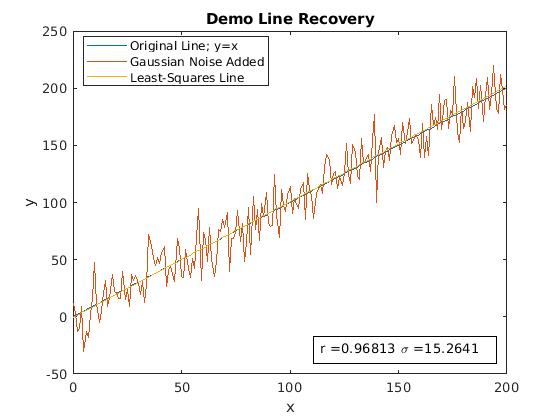
\includegraphics[width=\columnwidth]{demo.jpg}
            \caption{Regression Methods Applied to a Noisy $y=x$ with $\sigma = 16$}
            \label{fig:demo}
        \end{figure}
        \cref{fig:demo} Shows the results of the trial run of the used regression methods. We can see that the resulting line matches closely to the original and the correlation coefficient, being close to 1, indicates that this line is similar to the original. Furthermore, the retrieved standard deviation from this plot is fairly close to the standard deviation that was provided to the gaussian noise. Therefore we are able to conclude that the chosen methods work. 
        \begin{figure}[!ht]
            \centering
            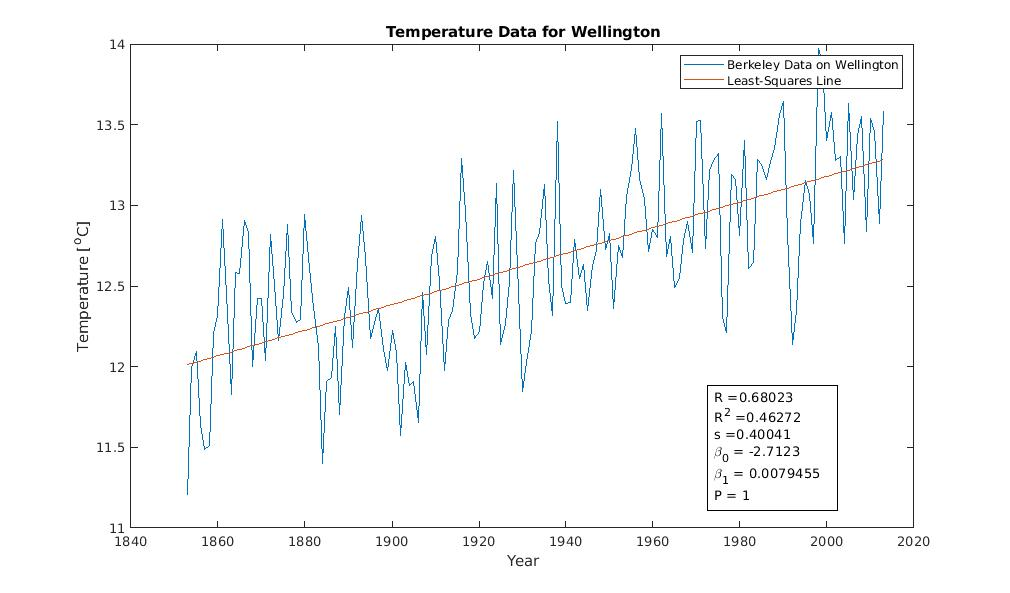
\includegraphics[width=\columnwidth]{regression.jpg}
            \caption{Regression Methods Applied to Wellington Temperature Data}
            \label{fig:regression}
        \end{figure}
        \cref{fig:regression} shows the results of performing the same methods as performed above. From this we can see that there is in fact a positive trend and that the year and temperature are reasonably positively correlated with a $r = 0.68023$. This indicates that the average temperature in wellington is gradually increasing each year.
        \begin{equation}
            \label{eq:U}
            U = \frac{r\sqrt{n-2}}{\sqrt{1-r^2}}
        \end{equation}
        Next the hypothesis test is performed. For this, we are going to use \cref{eq:U}, which is t distributed and can be used as a way of performing the test of the correlation coefficient. Using the t distribution, as seen in \cref{fig:regression}, we get a P of 1. This indicates that we can fully reject the null hypothesis as this sits outside of the t curve entirely and any confidence intervals we would normally compare this P to. So it is possible to confirm, very confidently, that the average temperature is correlated to the year, whether that be a positive or negative relationship.
        \par
        Another thing \cref{fig:regression} shows is that the standard deviation of the temperature is $0.4004$ indicating that it doesn't vary by much, making the trend appear stronger. 
    \section{Conclusion}
        In conclusion, the world is on fire and will slowly cook us alive if we don't take early action to reduce the temperature of the planet. The regression methods were certainly useful, however, I am not entirely certain that the method used for obtaining the standard devitation. Although it appears correct, based off multiple reruns of the program resulting in values between 15 and 17 for a provided standard deviation of 16, there are other equations used in the lecture slides to come to many different expressions for the standard deviation. The equation used in this report is even used in them, indicating that it may not be the actual standard deviation of the plot, but more, a stepping stone to get to the estimate. Additionally, I could not get the 95\% confidence intervals working as they appeared at temperatures of -188, which is clearly not right as that is an unlikely temperature to reach unless we were in an iceage, which I'm fairly confident we are currently not. So this method would need some more tweaking to be able to show those confidence intervals. 

    \bibliography{bibliography}
    \bibliographystyle{IEEEtran}

    \begin{appendices}
        \section{Regression Testing Code}
            \lstinputlisting{../nonTrivialData.m}
        \section{MATLAB Code}
            \lstinputlisting{../lab5.m}
    \end{appendices}
\end{document}